\documentclass{article}
\usepackage[spanish]{babel} %Definir idioma español
\usepackage[utf8]{inputenc} %Codificacion utf-8
\usepackage{amssymb, amsmath, amsbsy, wasysym}
\usepackage{multirow} % para tablas
\usepackage{graphicx}
\usepackage[dvipsnames]{xcolor}
\title{Práctica 7}
\author{Emmanuel Peto Gutiérrez}
\begin{document}
\maketitle

\section{Introducción}

\begin{itemize}

\item Sea $X$ un conjunto no vacío de de aristas de $G$. Una {\bf subgráfica inducida} por $X$ es la subgráfica minimal de $G$ con conjunto de aristas $X$ y se denota $\langle X \rangle$, esto es, $\langle X \rangle$ consiste de aquellos vértices de $G$ incidentes en al menos una arista de $X$. Una subgráfica $H$ de $G$ se llama {\bf subgráfica inducida por aristas} si $H = \langle X \rangle$ para algún conjunto no vacío de aristas $X$.

\item Una gráfica es {\bf n-regular} si todos los vértices en $G$ tienen grado $n$.

\item Un {\bf apareamiento} en una gráfica $G$ es una subgráfica 1-regular de $G$, esto es, una subgráfica inducida por una colección de aristas no adyacentes.

\item Sea $G$ una gráfica y sea $M$ un apareamiento maximal para $G$. Ya que $M$ es un apareamiento, sus aristas no tienen vértices en común, y como $M$ es maximal, todas las otras aristas tienen un vértice en común con al menos una de las aristas en $M$.

\item Una {\bf cobertura de vértices} de una gráfica $G$ es un subconjunto $V' \subseteq V$ tal que si $(u,v) \in E$, entonces $u \in V'$ o $v \in V'$(o ambos).

\item {\bf Teorema:} El conjunto de vértices incidentes a las aristas de un apareamiento maximal $M$ es una cubierta de vértices con no más de dos veces el número de vértices de una cubierta óptima.

\end{itemize}

En la figura \ref{grafica1} se muestra el apareamiento $\{(v_2 , v_3),(v_5 , v_4)\}$. Los vértices $v_2 , v_3 , v_4$ y $v_5$ forman una cobertura de vértices.

\begin{figure}[htbp]
\centering
\includegraphics[scale=1.5]{g1}
\caption{Las aristas rojas forman un apareamiento.}
\label{grafica1}
\end{figure}

\section{Descripción}

Esta práctica consiste en implementar un algoritmo de aproximación que genere una posible solución para el problema de Cubierta de Vértices dada una gráfica $G$.

Dicho programa debe garantizar encontrar una Cubierta de Vértices que contenga no más del doble de vértices de la cubierta óptima.

\subsection{Entrada}

El programa debe recibir como entrada el nombre del archivo con la información necesaria para construir la gráfica $G$. Esto es:

$\bullet$ En la primera línea, los vértices de la gráfica separados por ``,''.

$\bullet$ De la segunda línea en adelante, pares de vértices separados por ``,'' que indican las aristas de la gráfica.

\subsection{Salida}

El programa debe imprimir en consola el conjunto de vértices pertenecientes a la cubierta obtenida.

\section{Extra}

Obtendrán un punto extra si pintan de rojo los vértices que pertenecen a la cobertura.

\section{Entrega}

\begin{itemize}
\item Deben entregarlo como un archivo comprimido de una carpeta con el mismo nombre.
\item La carpeta debe ser: \textbf{Practica7\_ApellidopaternoApellidomaterno}. Por ejemplo \textbf{Practica7\_PetoGutierrez}.
\item Su carpeta debe contener un archivo \emph{readme} que contenga: número de cuenta, nombre completo, 
correo y las instrucciones para compilar y ejecutar su programa(se recomienda un \emph{Makefile}).
\item Si su carpeta contiene un ejecutable(como *.jar) enviarlo como un enlace de dropbox o drive.
\item El asunto debe ser: \textbf{[AAlgoritmos]Practica7}.
\item El correo al que enviarán la práctica es: \emph{empg014@ciencias.unam.mx}
\end{itemize}

La fecha de entrega es el \textbf{4 de diciembre}.

\end{document}


